\documentclass{article}
\usepackage[utf8]{inputenc}
\usepackage{amsmath}
\usepackage{hyperref}
\usepackage[pdftex]{graphicx}

\newcommand{\HRule}{\rule{\linewidth}{0.5mm}}
\newcommand{\tab}[1]{\hspace{.2\textwidth}\rlap{#1}}

\begin{document}
\begin{titlepage}
	\begin{center}
		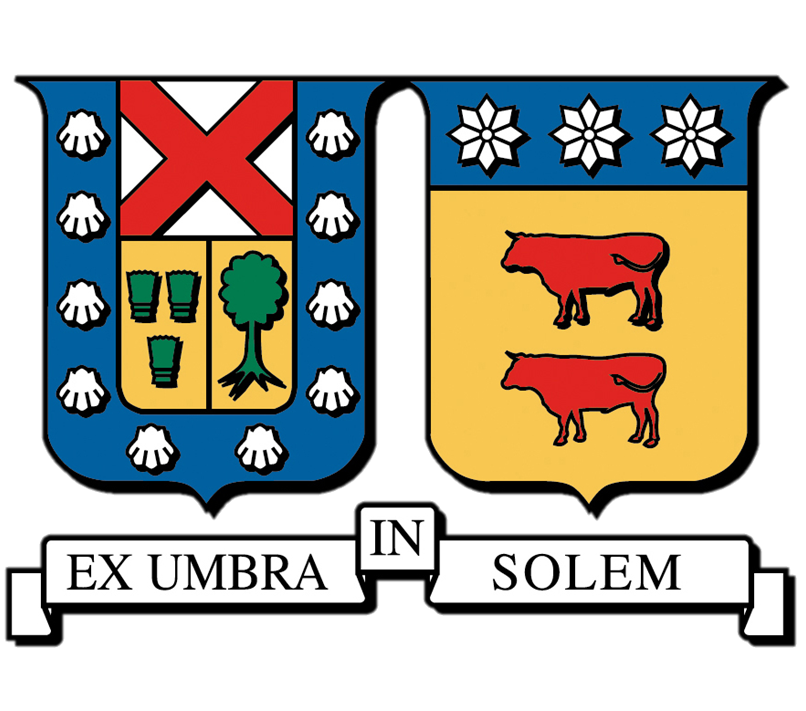
\includegraphics[width=0.30\textwidth]{Logo_UTFSM.png}~\\[1cm]
		\textsc{\LARGE Universidad Técnica Federico Santa María.}\\[1.2cm]
		\textsc{\Large Sistemas de Gestión.}\\[0.2cm]
		\textsc{\Large Departamento de Informática.}\\[0.2cm]
	
		% Title
		\HRule \\[0.4cm]
		{ \huge \bfseries Cuando Steve Jobs comía caramelos.\\[0.4cm] }
		\HRule \\[1.5cm]
		
		% Author and supervisor
		\begin{minipage}{0.9\textwidth}
			\begin{flushleft} \large
				\emph{Resumen:} \\
				Steve Jobs no nacio siendo un calvo, en algún momento fue un niño
				lleno de sueños e ilusiones, la mayoria de ellas repletas de caramelos.
			\end{flushleft}
			\begin{flushright} 
				\emph{Palabras clave:} Steve Jobs, Debate.
			\end{flushright}
		\end{minipage}
		\vfill
	
		% Bottom of the page
		{\large Hernán Vargas Leighton.\\
		\href{mailto:hernan.vargas@alumnos.usm.cl}{hernan.vargas@alumnos.usm.cl}
		\\[0.2cm] \today }
	\end{center}
\end{titlepage}
\end{document}
